\begin{figure}[h]
    \centering
    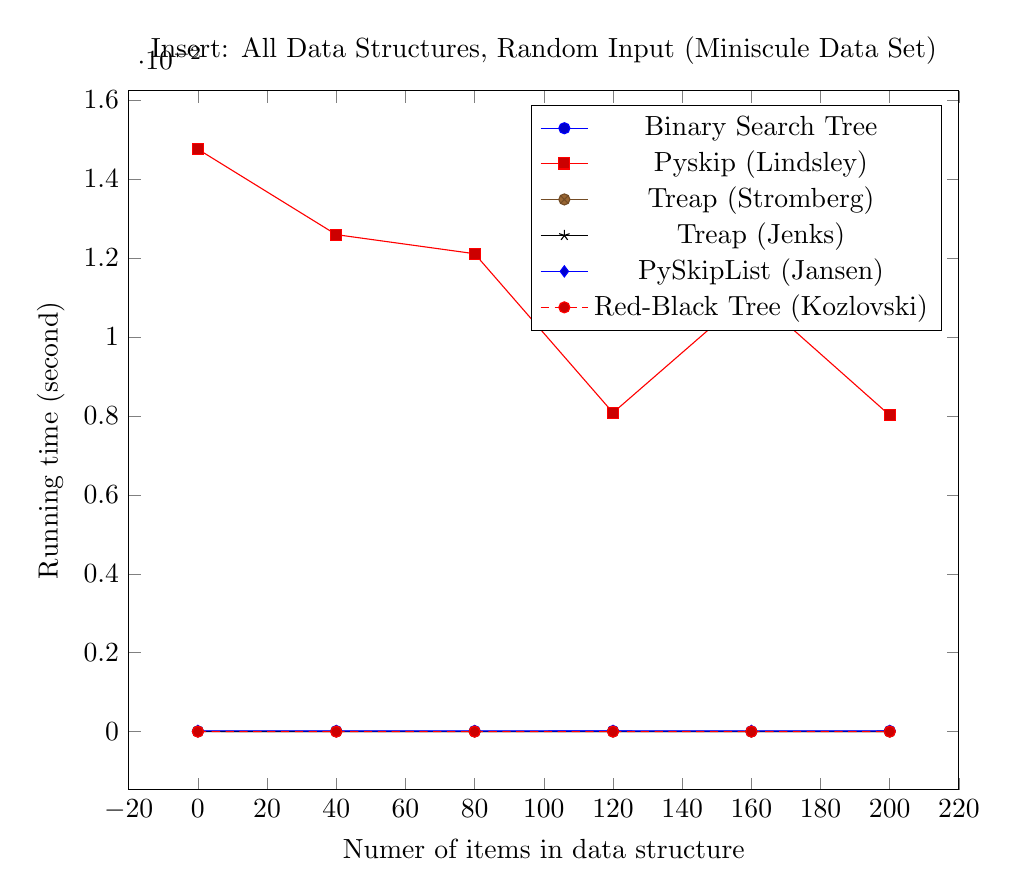
\begin{tikzpicture}
        \begin{axis}[
            xlabel={Numer of items in data structure},
            ylabel={Running time (second)},
            title={Insert: All Data Structures, Random Input (Miniscule Data Set)},
            width=\textwidth
        ]
		\addplot coordinates {
			(0, 1.1595250464857543e-05)
			(40, 1.695617145927031e-05)
			(80, 1.6022527915104945e-05)
			(120, 1.834157800821856e-05)
			(160, 1.0480901718956659e-05)
			(200, 1.7950050070325574e-05)
		};
		\addplot coordinates {
			(0, 0.014754549629930835)
			(40, 0.012590544600302778)
			(80, 0.012107097949748891)
			(120, 0.008079721111638172)
			(160, 0.01112433270839439)
			(200, 0.008014185358361025)
		};
		\addplot coordinates {
			(0, 7.710088620882516e-06)
			(40, 5.270568393100916e-06)
			(80, 4.276689781868015e-06)
			(120, 4.336924849290824e-06)
			(160, 5.330803460523726e-06)
			(200, 5.180215792144338e-06)
		};
		\addplot coordinates {
			(0, 2.7105780306513337e-06)
			(40, 2.4094026940701953e-06)
			(80, 2.1985799582679986e-06)
			(120, 2.3190500929359813e-06)
			(160, 2.0781098236000163e-06)
			(200, 2.6202254298723916e-06)
		};
		\addplot coordinates {
			(0, 2.1443683976585247e-05)
			(40, 1.9365574153162868e-05)
			(80, 1.8040402671459788e-05)
			(120, 1.981733715830103e-05)
			(160, 1.9636631956210238e-05)
			(200, 1.8642753344977338e-05)
		};
		\addplot coordinates {
			(0, 2.770813098074143e-06)
			(40, 2.9816358338763393e-06)
			(80, 3.102105968544322e-06)
			(120, 3.4936339064373103e-06)
			(160, 3.4635163725482697e-06)
			(200, 3.4635163725482697e-06)
		};
        \legend{Binary Search Tree, Pyskip (Lindsley), Treap (Stromberg), Treap (Jenks), PySkipList (Jansen), Red-Black Tree (Kozlovski)}
        \end{axis}
    \end{tikzpicture}
    \caption{Average of 10 operations, benchmarked every 40, starting at 0.}
\end{figure}